\documentclass{beamer}
%
% Choose how your presentation looks.
%
% For more themes, color themes and font themes, see:
% http://deic.uab.es/~iblanes/beamer_gallery/index_by_theme.html
%
\mode<presentation>
{
  \usetheme{Madrid}      % or try Darmstadt, Madrid, Warsaw, ...
  \usecolortheme{beaver} % or try albatross, beaver, crane, ...
  \usefonttheme{serif}  % or try serif, structurebold, ...
  \setbeamertemplate{navigation symbols}{}
  \setbeamertemplate{caption}[numbered]
}
\renewcommand{\arraystretch}{2}
\usepackage[utf8]{inputenc}
\usepackage[spanish]{babel}
\usepackage{xcolor}
\usepackage{graphicx}
\usepackage{amsfonts}
\usepackage{subcaption}
\usepackage{amssymb}
\usepackage{mathtools}
\usepackage{amsmath}
\usepackage{beton}
\usepackage{hyperref}

\usepackage{euler}
\usepackage[T1]{fontenc}
\usepackage{listings}
\usepackage{multicol}
\lstset
{
    language=[LaTeX]TeX,
    breaklines=true,
    basicstyle=\tt\scriptsize,
    %commentstyle=\color{green}
    keywordstyle=\color{blue},
    %stringstyle=\color{black}
    identifierstyle=\color{magenta},
}

\title[Administración GNU/Linux]{Administración de Sistemas Operativos GNU/Linux}
\author{Lino Ontano}
%\institute{ESPOL}
\date{Abril 8, 2019}

\AtBeginSection[]
{
  \begin{frame}<beamer>
    \frametitle{Contenido}
    \tableofcontents[currentsection]
  \end{frame}
}

\AtBeginSubsection[]
{
  \begin{frame}
    \frametitle{Contenido}
    \tableofcontents[currentsection,currentsubsection]
  \end{frame}
}


\begin{document}

\begin{frame}
  \titlepage
\end{frame}

% Uncomment these lines for an automatically generated outline.
\begin{frame}{Contenido}
  \tableofcontents
\end{frame}

\section{Módulo 1}
\subsection{Sistemas Operativos Linux: Estructura e Instalación}
\begin{frame}{GNU/Linux}
\begin{figure}
	
\includegraphics[height=2.7cm]{img/Gnulinux.png}
\end{figure}
\begin{itemize}
\item Sistema operativo libre tipo Unix; multiplataforma, multiusuario y multitarea.
\item Combinación de varios proyectos: GNU y el núcleo Linux (kernel).
\item Existen derivados de Linux que no tienen componentes GNU (Android) y viceversa (Debian GNU/Hurd)
\item GNU/Linux se encuentran en compendios conocidos como distribuciones o \textit{distros}.
\end{itemize}
\end{frame}
\begin{frame}{FHS}
\begin{itemize}
    \item \textbf{Filesystem Hierarchy Standard}: estándar de jerarquía del sistema de archivos. 
    \item Todos los archivos y directorios aparecen bajo el directorio raíz, /, aun cuando se encuentren en distintos dispositivos físicos.
\end{itemize}

\end{frame}
\begin{frame}{Estructura GNU/Linux}
\begin{figure}
	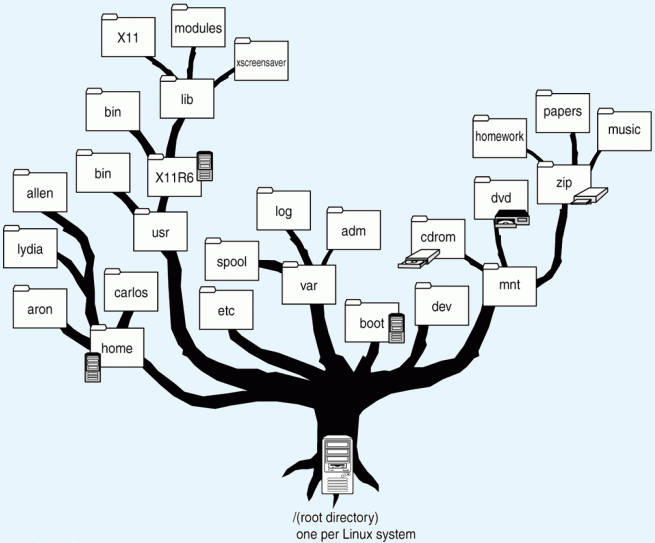
\includegraphics[height=7cm]{img/estructura.jpg}
\end{figure}
\end{frame}

\begin{frame}{Directorios principales}
\begin{itemize}
\item \textbf{/ :} es el nivel más alto dentro de la jerarquía de directorios.
\item \textbf{/bin:} aplicaciones binarias de comandos esenciales para una sesión de usuario único o mutliusuario (Incluyen por ejemplo cat, ls, cp, rm, etc).
\item \textbf{/sbin: }sistema de binarios esencial, comandos y programas exclusivos del superusuario (Por ejemplo init, route, ifup).
\item \textbf{/dev:} permite interactuar con los dispositivos del equipo.
\item \textbf{/etc:} archivos de configuración del sistema específico del Host de todo el sistema. 
\item \textbf{/home:} carpeta por defecto de los usuarios.
\item \textbf{/tmp:} almacena ficheros temporales.
\item \textbf{/root:} directorio home del usuario root. 
\item \textbf{/mnt:} sistema de archivos montados temporalmente. Discos duros y particiones de forma temporal en el sistema.
\end{itemize}
\end{frame}
\begin{frame}{Instalación}
\begin{multicols}{2}
\centering
\begin{figure}
	
\includegraphics[height=3cm]{img/rhel.png}
\end{figure}
\textbf{Red Hat} Enterprise Linux 7.4
\begin{figure}
	
\includegraphics[height=3cm]{img/Virtualbox.png}
\end{figure}
\textbf{ \href{https://download.virtualbox.org/virtualbox/6.0.4/VirtualBox-6.0.4-128413-Win.exe}{Oracle VirtualBox}}

\end{multicols}

\end{frame}
\subsection{Comandos básicos para administración de archivos y directorios}
\subsection{Gestión y administración de usuarios y grupos}
\subsection{Gestión, administración e instalación de procesos/paquetes RPM}
\subsection{Empaquetado y compresión de archivos y directorios}
%meter aqui TIPO DE SISTEMAS DE FICHEROS con compresion y eso
\section{Módulo 2}


% \subsection{Tables and Figures}

% \begin{frame}{Tables and Figures}

% \begin{itemize}
% \item Use \texttt{tabular} for basic tables --- see Table~\ref{tab:widgets}, for example.
% \item You can upload a figure (JPEG, PNG or PDF) using the files menu.
% \item To include it in your document, use the \texttt{includegraphics} command (see the comment below in the source code).
% \end{itemize}

% Commands to include a figure:
%\begin{figure}
%\includegraphics[width=\textwidth]{your-figure's-file-name}
%\caption{\label{fig:your-figure}Caption goes here.}
%\end{figure}

% \begin{table}
% \centering
% \begin{tabular}{l|r}
% Item & Quantity \\\hline
% Widgets & 42 \\
% Gadgets & 13
% \end{tabular}
% \caption{\label{tab:widgets}An example table.}
% \end{table}

% \end{frame}

% \subsection{Mathematics}

% \begin{frame}{Readable Mathematics}

% Let $X_1, X_2, \ldots, X_n$ be a sequence of independent and identically distributed random variables with $\text{E}[X_i] = \mu$ and $\text{Var}[X_i] = \sigma^2 < \infty$, and let
% $$S_n = \frac{X_1 + X_2 + \cdots + X_n}{n}
%       = \frac{1}{n}\sum_{i}^{n} X_i$$
% denote their mean. Then as $n$ approaches infinity, the random variables $\sqrt{n}(S_n - \mu)$ converge in distribution to a normal $\mathcal{N}(0, \sigma^2)$.

% \end{frame}

\section{Módulo 3}


\end{document}
